
\documentclass[10 pt,usenames,dvipsnames, oneside]{article}
\usepackage{../../modelo-fracoes}
\graphicspath{{../../../Figuras/licao03/}}


\begin{document}

\begin{center}
  \begin{minipage}[l]{3cm}
\includegraphics[width=2cm]{../../../Figuras/logo}       
\end{minipage}\hfill
\begin{minipage}[r]{.8\textwidth}
 {\Large \scshape Atividade: Marque os números na reta}  
\end{minipage}
\end{center}
\vspace{.2cm}

\ifdefined\prof
%Caixa do Para o Professor
\begin{goals}
%Objetivos específicos
\begin{enumerate}
\item       Representar frações na reta numérica.
\item       Comparar frações.
\end{enumerate}

\tcblower

%Orientações e sugestões
\begin{itemize}
\item  A associação das frações aos pontos correspondentes exigirá estratégias e comparações variadas. Procure identificar e discutir as argumentações apresentadas pelos alunos.
\item  Inicialmente os alunos precisam identificar que as marcações em destaque identificam oitavos. Assim, por exemplo, para identificar quartos, será necessário reunir dois oitavos e para marcar   $\frac{3}{2}$   será necessário contar 12 oitavos.
\item  Esta atividade oferece também, de forma indireta, a oportunidade de os alunos estabelecerem comparações. Por exemplo, reconhecer que   $\frac{3}{4}$   é menor do que 1, que   $\frac{5}{4}$   é maior do que   $\frac{8}{4}$   = 2 e que   $\frac{10}{4}$   é menor do que   $\frac{10}{8}$  . Destaque e discuta essas e outras comparações com os seus alunos.
\end{itemize}
\end{goals}

\bigskip
\begin{center}
{\large \scshape Atividade}
\end{center}
\fi

Na reta numérica já estão marcados os números 0, 1 e $\frac{1}{2}$. Marque $\frac{3}{2}$, $\frac{3}{4}$, $\frac{5}{4}$, $\frac{8}{4}$, $\frac{10}{4}$, $\frac{1}{8}$, $\frac{7}{8}$, $\frac{10}{8}$ e 2.

\begin{center}
\begin{tikzpicture}[x=5mm,y=5mm]
\draw[->]  (-0.5,0) -- (26,0);
\draw  (0,-3pt) -- (0,3pt);
\draw  (1.25,-3pt) -- (1.25,3pt);
\draw  (2.5,-3pt) -- (2.5,3pt);
\draw  (3.75,-3pt) -- (3.75,3pt);
\draw  (5,-3pt) -- (5,3pt);
\draw  (6.25,-3pt) -- (6.25,3pt);
\draw  (7.5,-3pt) -- (7.5,3pt);
\draw  (8.75,-3pt) -- (8.75,3pt);
\draw  (10,-3pt) -- (10,3pt);
\draw  (11.25,-3pt) -- (11.25,3pt);
\draw  (12.5,-3pt) -- (12.5,3pt);
\draw  (13.75,-3pt) -- (13.75,3pt);
\draw  (15,-3pt) -- (15,3pt);
\draw  (16.25,-3pt) -- (16.25,3pt);
\draw  (17.5,-3pt) -- (17.5,3pt);
\draw  (18.75,-3pt) -- (18.75,3pt);
\draw  (20,-3pt) -- (20,3pt);
\draw  (21.25,-3pt) -- (21.25,3pt);
\draw  (22.5,-3pt) -- (22.5,3pt);
\draw  (23.75,-3pt) -- (23.75,3pt);
\draw  (25,-3pt) -- (25,3pt);

\node[below] at (0,0) {0};
\node[below] at (5,0) {$\frac{1}{2}$};
\node[below] at (10,0)  {1};
\end{tikzpicture}
\end{center}

\ifdefined\prof
\begin{solucao}

\begin{center}
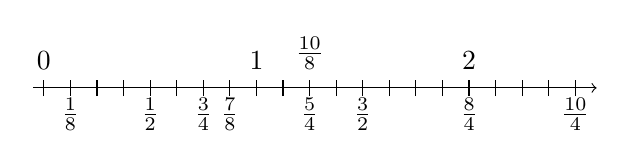
\begin{tikzpicture}[x=1cm,y=1cm,xscale=.27]
\draw[->]  (-.5,0) -- (26,0);
\draw  (0,-3pt) -- (0,3pt);
\draw  (1.25,-3pt) -- (1.25,3pt);
\draw  (2.5,-3pt) -- (2.5,3pt);
\draw  (3.75,-3pt) -- (3.75,3pt);
\draw  (5,-3pt) -- (5,3pt);
\draw  (6.25,-3pt) -- (6.25,3pt);
\draw  (7.5,-3pt) -- (7.5,3pt);
\draw  (8.75,-3pt) -- (8.75,3pt);
\draw  (10,-3pt) -- (10,3pt);
\draw  (11.25,-3pt) -- (11.25,3pt);
\draw  (12.5,-3pt) -- (12.5,3pt);
\draw  (13.75,-3pt) -- (13.75,3pt);
\draw  (15,-3pt) -- (15,3pt);
\draw  (16.25,-3pt) -- (16.25,3pt);
\draw  (17.5,-3pt) -- (17.5,3pt);
\draw  (18.75,-3pt) -- (18.75,3pt);
\draw  (20,-3pt) -- (20,3pt);
\draw  (21.25,-3pt) -- (21.25,3pt);
\draw  (22.5,-3pt) -- (22.5,3pt);
\draw  (23.75,-3pt) -- (23.75,3pt);
\draw  (25,-3pt) -- (25,3pt);

\node[above] at (0,3pt)  {0};
\node[below] at (5,0) {$\frac{1}{2}$};
\node[above] at (10,3pt)  {1};
\node[below] at (15,0) {$\frac{3}{2}$};
\node[below] at (7.5,0) {$\frac{3}{4}$};
\node[below] at (12.5,0) {$\frac{5}{4}$};
\node[below] at (20,0) {$\frac{8}{4}$};
\node[above] at (20,3pt) {2};
\node[below] at (25,0) {$\frac{10}{4}$};
\node[below] at (1.25,0) {$\frac{1}{8}$};
\node[below] at (8.75,0) {$\frac{7}{8}$};
\node[above] at (12.5,3pt) {$\frac{10}{8}$};
\end{tikzpicture}
\end{center}

\end{solucao}
\fi

\end{document}